\documentclass[]{article}
\newcommand{\FileDepth}{../../..}
\usepackage[letterpaper, landscape, margin=0.5cm]{geometry}
\usepackage[T1]{fontenc}
\usepackage{textcomp}%Not strictly necessary, but gives \textmu command for "micro."
\usepackage{fancyhdr}
\usepackage{amsmath}
\usepackage{amssymb}
\usepackage{graphicx}
\usepackage{xcolor}
\usepackage{tikz}
\usetikzlibrary{calc}
\usepackage[shortlabels]{enumitem}
\usepackage{multicol}
\usepackage{vwcol}
\usepackage{hyperref}
\usepackage{wrapfig}
%opening
\newcommand{\SecType}{S}
\newcommand{\Week}{8}
\title{PH 211 Studio \Week}
\author{Benjamin Bauml}
\date{Summer 2024}

\newcommand{\Purpose}{4}
\newcommand{\DefOnly}{0}

% Version 2024-06-14
% Changes
% 2024-02-21 Added xstring package to enable smooth implementation of new \ModePage command.
% 2024-04-27 Set up to split activities and formatting aspects into separate files. Removed dependence on xcomment. Added an automatic counter to number the activities in a problem set.
% 2024-05-19 Revised old format for \TeachingTips command, which did not support \DefOnly.
% 2024-06-14 Added Repurpose environment to allow mixing of different purpose levels in the same document.
\usepackage{tcolorbox}
\usepackage{xstring}
% You will want the following four lines in your document (the last two uncommented):
% For Assignment, leave Purpose as 1. For Worksheet, set to 2. For Student Solution, set to 3. For Teacher Solution, set to 4.
% If you want keep the pieces from being called manually, set DefOnly to 0.
%\newcommand{\Purpose}{4}
%\newcommand{\DefOnly}{1}
\newcommand{\Exclusion}{0}
\newcommand{\PageTurn}{0}
\newcommand{\GrayProb}{0}
\newcommand{\Tipsy}{0}

% Assignment
\if\Purpose1
\renewcommand{\Exclusion}{1}
\fi
% Worksheet
\if\Purpose2
\renewcommand{\Exclusion}{1}
\renewcommand{\PageTurn}{1}
\fi
% Student Solution
\if\Purpose3
\renewcommand{\PageTurn}{1}
\renewcommand{\GrayProb}{1}
\fi
% Teaching Copy
\if\Purpose4
\renewcommand{\PageTurn}{1}
\renewcommand{\GrayProb}{1}
\renewcommand{\Tipsy}{1}
\fi

\newenvironment{Repurpose}[1]{
\renewcommand{\Purpose}{#1}
\renewcommand{\Exclusion}{0}
\renewcommand{\PageTurn}{0}
\renewcommand{\GrayProb}{0}
\renewcommand{\Tipsy}{0}
% Assignment
\if\Purpose1
\renewcommand{\Exclusion}{1}
\fi
% Worksheet
\if\Purpose2
\renewcommand{\Exclusion}{1}
\renewcommand{\PageTurn}{1}
\fi
% Student Solution
\if\Purpose3
\renewcommand{\PageTurn}{1}
\renewcommand{\GrayProb}{1}
\fi
% Teaching Copy
\if\Purpose4
\renewcommand{\PageTurn}{1}
\renewcommand{\GrayProb}{1}
\renewcommand{\Tipsy}{1}
\fi
}{}

\def \NewQ {0}
\def \PForce {0}
\newcommand{\MaybePage}[1]{
	\def \PForce {#1}
	\if\PForce1
	\newpage
	\else
	\if\NewQ0
	\gdef \NewQ {\PageTurn}
	\else
	\newpage
	\fi
	\fi
}

\newcommand{\ModePage}[1]{
	\IfSubStr{#1}{\Purpose}{\newpage}{}
}

\newcounter{ActNumber}
\setcounter{ActNumber}{0}

\newcommand{\Problem}[4][0]{%The first argument is optional, and if it is set to 1, the \newpage will be forced. The second argument is the name of the activity, the third is the command the activity is stored as, and the fourth is the actual problem statement.
\newcommand{#3}{
\MaybePage{#1}
\addtocounter{ActNumber}{1}
\section*{\SecType\Week-\theActNumber: #2}
\if\GrayProb1
\begin{tcolorbox}[colback=lightgray,colframe=lightgray,sharp corners,boxsep=1pt,left=0pt,right=0pt,top=0pt,bottom=0pt,after skip=2pt]
\else
\begin{tcolorbox}[colback=white,colframe=white,sharp corners,boxsep=1pt,left=0pt,right=0pt,top=0pt,bottom=0pt,after skip=2pt]
\fi
#4
\end{tcolorbox}\noindent
}
\if\DefOnly0
\else
#3
\fi
}
	
\newcommand{\ProblemSub}[3][0]{%The first argument is optional, and if a string of numbers is entered into it, it will force a \newpage in any \Purpose that shows up in the string. For example, "13" would lead to the newpage being forced in modes 1 and 3. The second is the command the activity is stored as, and the third is the actual problem statement.
\newcommand{#2}{
\ModePage{#1}
\if\GrayProb1
\begin{tcolorbox}[colback=lightgray,colframe=lightgray,sharp corners,boxsep=1pt,left=0pt,right=0pt,top=0pt,bottom=0pt,after skip=2pt]
\else
\begin{tcolorbox}[colback=white,colframe=white,sharp corners,boxsep=1pt,left=0pt,right=0pt,top=0pt,bottom=0pt,after skip=2pt]
\fi
#3
\end{tcolorbox}\noindent
}
\if\DefOnly0
\else
#2
\fi
}
		
\newcommand{\Solution}[2]{%The first argument is the command the solution is stored as, and the second is the actual solution.
\newcommand{#1}{
\if\Exclusion0
#2
\fi
}
\if\DefOnly0
\else
#1
\fi
}
		
\newcommand{\ProblemFig}[2]{%The first argument is the command the figure is stored as, and the second is the actual figure.
\newcommand{#1}{
\begin{figure}[h]
#2
\end{figure}
}
\if\DefOnly0
\else
#1
\fi
}

\newcommand{\TeachingTips}[2]{%The first argument is the command the tip is stored as, and the second is the actual tip.
\newcommand{#1}{
\if\Tipsy1
\begin{tcolorbox}[colback=lightgray,colframe=black]
#2
\end{tcolorbox}
\fi
}
\if\DefOnly0
\else
#1
\fi
}
\usepackage[absolute]{textpos}
% This package relies on Assignment Format 2024-06-14 or later to work. It is recommended that the Purpose and DefOnly commands be given as such:
%\newcommand{\Purpose}{4}
%\newcommand{\DefOnly}{0}
% Activities need to be entered outside of the TeacherMargin and PresentSpace environments, otherwise they will be defined only locally. They can even go in the preamble.
\newenvironment{TeacherMargin}{\begin{textblock*}{10.8cm}(0.5cm,0.5cm)
\small}{\end{textblock*}
\hspace{0.1cm}}
\newenvironment{PresentSpace}{\begin{textblock*}{0.3cm}(26.85cm,9.35cm)
--
\end{textblock*}
\begin{textblock*}{0.3cm}(26.85cm,18.7cm)
--
\end{textblock*}
\begin{textblock*}{0.3cm}(26.85cm,12.24cm)
	--
\end{textblock*}
\begin{textblock*}{15.6cm}(11.8cm,0.5cm)
\begin{Repurpose}{1}
\Large}{\end{Repurpose}
\end{textblock*}
\hspace{0.1cm}}

%\newcommand{\FBDaxes}[3]{
	\begin{scope}[shift={(#1)},rotate=#2]
		% x-axis
		\draw[thick,->] (-2,0) -- (2,0);
		\node[anchor=west] at (2,0) {$x$};
		% y-axis
		\draw[thick,->] (0,-2) -- (0,2);
		\node[anchor=west] at (0,2) {$y$};
		\coordinate (#3) at (0,0);
	\end{scope}
}
\newcommand{\FBDvectorMA}[4]{
	\begin{scope}[shift={(#1)}]
		\coordinate (#4tip) at ({#2*cos(#3)},{#2*sin(#3)});
		\draw[ultra thick,blue,->] (#1) -- (#4tip);
	\end{scope}
}
\newcommand{\FBDvectorXY}[3]{
	\begin{scope}[shift={(#1)}]
		\coordinate (#3tip) at (#2);
		\draw[ultra thick,blue,->] (0,0) -- (#3tip);
	\end{scope}
}
\newcommand{\FBDdot}[1]{
	\filldraw[black] (#1) circle (3pt);
}
%\newcommand{\MVec}[3][0]{%Creates a momentum vector of length #3 centered at #2 and rotated #1 degrees counterclockwise.
	\begin{scope}[rotate=#1,shift={(#2)}]
		\draw[->,thick] ({-#3/2},0) -- ({#3/2},0);
	\end{scope}
}
\newcommand{\MDot}[1]{%Creates a dot at #1 to represent a zero vector.
	\filldraw (#1) circle (1pt);
}
\newcommand{\MVDRows}[2][4.5]{%Creates the rows (initial, delta, final) of a momentum vector diagram. The optional argument determines the width of the table, and defaults to a good length for three columns (two objects and the total system). The non-optional argument gives a coordinate name (not displayed) to the diagram.
	\begin{scope}
		%\draw[thick] (0,5.5) -- (0,0);
		\draw[thick] (-1,4.5) -- (#1,4.5);
		\node at (-0.5,3.75) {$\vec{p}_{i}$};
		\draw[thick] (-1,3) -- (#1,3);
		\node at (-0.5,2.25) {$\Delta\vec{p}$};
		\draw[thick] (-1,1.5) -- (#1,1.5);
		\node at (-0.5,0.75) {$\vec{p}_{f}$};
		\coordinate (#2) at (0,5);
	\end{scope}
}
\newcommand{\MVDCol}[4][0.75]{%Creates a column for an object in a momentum vector diagram. The first (non-optional) argument is the coordinate name (not displayed) of the column, while the second is the displayed column header. The first argument also names the three entries down the column. The third argument anchors the column, so it should either be the coordinate name of the MVD (for the first column) or the coordinate name of the previous column. The optional argument indicates how far the center of the column should be from the previous column's edge, and defaults to 0.75
	\begin{scope}[shift={(#4)}]
		\node at (#1,0) {#3};
		%\draw[thick] ({#1*2},0.5) -- ({#1*2},-5);
		\draw[thick] (0,0.5) -- (0,-5);
		\coordinate (#2init) at (#1,-1.25);
		\coordinate (#2delt) at (#1,-2.75);
		\coordinate (#2fin) at (#1,-4.25);
		\coordinate (#2) at ({#1*2},0);
	\end{scope}
}

%\input{\FileDepth/Activities/Activity_One/Activity_One.tex}
%\input{\FileDepth/Activities/Activity_Two/Activity_Two.tex}

\begin{document}
\begin{TeacherMargin}
\noindent\textbf{Energy is (C)} \\
The work-energy theorem ($W_{\text{net,ext}} = \Delta E_{\text{total}}$) determines whether energy is conserved. Everything that can do significant amounts of work is in our system. \\
\textbf{Momentum is (B)} \\
The impulse-momentum theorem ($\int_{t_{i}}^{t_{f}}\vec{F}^{net}dt = \vec{J}_{net} = \Delta\vec{p}$) determines whether momentum is conserved. Everything that exerts a significant force is in our system.
\end{TeacherMargin}
\begin{PresentSpace}
\begin{center}
	\huge Studio 8: Combining Physics Concepts I \\
	\vspace{0.5cm}
\end{center}
\underline{Warm-Up Activity}
\begin{itemize}
	\item A tennis ball and a basketball are dropped from a \\
	height $h$ as shown.
	\item Our system is the tennis ball, the basketball, and \\
	the Earth.
\end{itemize}
Energy/Momentum is \dots \\
(answer twice; once for energy and once for momentum)
\begin{enumerate}[(A)]
	\item \dots conserved, because energy/momentum is \\
	\phantom{\dots}always conserved.
	\item \dots conserved, because the net force on the system is zero.
	\item \dots conserved, because the work done on the system is zero.
	\item \dots not conserved, because energy is never conserved.
	\item \dots not conserved, because the net force on the system is not zero.
	\item \dots not conserved, because the work done on the system is not zero.
\end{enumerate}
\begin{comment}{2}
Energy is\dots
\begin{enumerate}[(A)]
	\item \dots conserved, because energy is always conserved.
	\item \dots conserved, because the net force on the system is zero.
	\item \dots conserved, because the work done on the system is zero.
	\item \dots not conserved, because energy is never conserved.
	\item \dots not conserved, because the net force on the system is not zero.
	\item \dots not conserved, because the work done on the system is not zero.
\end{enumerate}
\vspace{2cm}
Momentum is\dots
\begin{enumerate}[(A)]
	\item \dots conserved, \\
	because momentum \\
	is always \\
	conserved.
	\item \dots conserved, because the net force on the system is zero.
	\item \dots conserved, because the work done on the system is zero.
	\item \dots not conserved, because momentum is never conserved.
	\item \dots not conserved, because the net force on the system is not zero.
	\item \dots not conserved, because the work done on the system is not zero.
\end{enumerate}
\end{comment}
\end{PresentSpace}
\begin{textblock*}{4cm}(23cm,2cm)
\begin{center}
	\Huge
	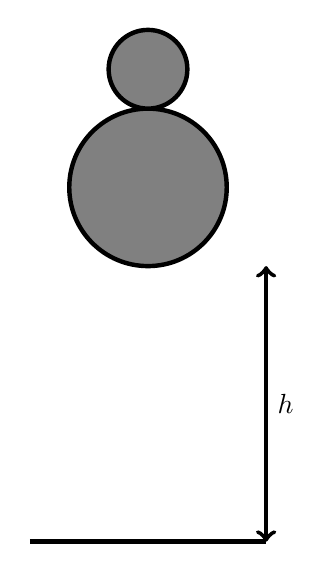
\begin{tikzpicture}
		\draw[ultra thick] (-1.5,0) -- (1.5,0);
		\draw[ultra thick,<->] (1.5,0) -- (1.5,1.75) node[anchor=west] {$h$} -- (1.5,3.5);
		\draw[ultra thick,color=black,fill=gray] (0,4.5) circle (1cm);
		\draw[ultra thick,color=black,fill=gray] (0,6) circle (0.5cm);
	\end{tikzpicture}
\end{center}
\end{textblock*}
\newpage
\begin{TeacherMargin}

\end{TeacherMargin}
\begin{PresentSpace}
\vspace{-10pt}
\section*{A Deeper Model for Interactions}
\vspace{-10pt}
\begin{itemize}
	\item Quantities
	\begin{itemize}
		\item Energy \qquad \qquad \qquad \quad \ \ $E$
		\item Work \qquad \qquad \qquad \quad \ \ \ \ $W = \int_{r_{i}}^{r_{f}}\vec{F}\cdot d\vec{r}$
		\item Kinetic Energy \qquad \qquad $K=\frac{1}{2}mv^{2}$
		\item Potential Energy \qquad \quad \ $U=$ depends on interaction \\
		You have to tell everyone where zero $PE$ is!
		\begin{itemize}
			\item Gravity \qquad $U_{g} = mgy$
			\item Spring \qquad \ $U_{sp} = \frac{1}{2}kx^{2}$
		\end{itemize}
		\item Momentum \qquad \qquad \qquad $\vec{p}=m\vec{v}$
		\item Impulse \qquad \qquad \quad \quad \ \ $\vec{J}_{net}=\int_{t_{i}}^{t_{f}}\vec{F}^{net}dt$
	\end{itemize}
	\item Laws
	\begin{itemize}
		\item Work-energy theorem \qquad $W_{\text{net,ext}} = \Delta E_{\text{total}}$
		\item Impulse-momentum theorem \qquad $\vec{J}_{net} = \Delta\vec{p}$
	\end{itemize}
\end{itemize}
\end{PresentSpace}
\newpage
\begin{TeacherMargin}
\begin{center}
\begin{tabular}{c||c|c|c|c||c}
	& $U_{gTB}$ & $K_{TB}$ & $U_{gBB}$ & $K_{BB}$ & $E_{\text{total}}$ \\ \hline
	$t_{i}$ & $mg(h+2R)$ & $0$ & $Mgh$ & $0$ & $mg(h+2R)+Mgh$ \\ \hline
	$t_{f}$ & $mgh_{max}$ & $0$ & $0$ & $0$ & $mgh_{max}$
\end{tabular}
\end{center}
\begin{align*}
	mgh_{max} & = mg(h+2R) + Mgh \\
	h_{max} & = h + 2R + \frac{M}{m}h \\
	& = \left(\frac{M}{m}+1\right)h+2R
\end{align*}
You don't necessarily need to include the radius of the basketball, as the tennis ball never gets lower than $2R$. If you leave off $2R$, you are effectively setting the zero of potential for the tennis ball at $2R$ above the ground, and so the $h_{max}$ you would find would actually be measured from this higher point. \\

\noindent Plugging in the given numbers, note that $\frac{M}{m}=15$, so $h_{max} = 8.23$ m. Now, this would exceed the ceiling height in our classroom, but when we actually do the demonstration, the non-negligible bounce of the basketball leads to this being a large overestimate; the tennis ball won't hit the ceiling after being dropped from this height. \\

\noindent However, if you wanted to find out the maximum drop height in the ideal case, it would only take a small rearrangement of the equation:
\begin{align*}
	h = \frac{h_{max}-2R}{\frac{M}{m}+1}.
\end{align*}
Assuming a ceiling height of 3 m, we should drop the ball from less than $h \approx 0.17$ m. In practice, this will be nowhere near the ceiling.
\end{TeacherMargin}
\begin{PresentSpace}
\vspace{-10pt}
\section*{S8-1: Ball Drop -- Height}
\vspace{-10pt}
\begin{itemize}
	\item A tennis ball and a basketball are dropped from a \\
	height $h$ as shown.
	\item Our system is the tennis ball, the basketball, and \\
	the Earth.
	\item If the basketball does not bounce at all, how high does the tennis ball go?
	\begin{itemize}
		\item Basketball Mass: $M=0.6$ kg
		\item Basketball Radius: $R \approx 11.5$ cm
		\item Tennis Ball Mass: $m=0.04$ kg
		\item Drop Height: $h=0.5$ m
	\end{itemize}
\end{itemize}
\end{PresentSpace}
\newpage
\begin{TeacherMargin}
\noindent Let us add two times to our table: $t_{bb}$ (right before the bounce) and $t_{ab}$ (right after the bounce).
\begin{center}
\begin{tabular}{c||c|c|c|c||c}
	& $U_{gTB}$ & $K_{TB}$ & $U_{gBB}$ & $K_{BB}$ & $E_{\text{total}}$ \\ \hline
	$t_{i}$ & $mg(h+2R)$ & $0$ & $Mgh$ & $0$ & $mg(h+2R)+Mgh$ \\ \hline
	$t_{bb}$ & $mg(2R)$ & $\frac{1}{2}mv_{bb}^{2}$ & $0$ & $\frac{1}{2}Mv_{bb}^{2}$ & $mg(2R) + \frac{1}{2}(m+M)v_{bb}^{2}$ \\ \hline
	$t_{ab}$ & $mg(2R)$ & $\frac{1}{2}mv_{ab}^{2}$ & $0$ & $0$ & $mg(2R) + \frac{1}{2}mv_{ab}^{2}$ \\ \hline
	$t_{f}$ & $mgh_{max}$ & $0$ & $0$ & $0$ & $mgh_{max}$
\end{tabular}
\end{center}
Note that the extra starting height of the tennis ball really doesn't matter in some of these calculations. It drops the same height as the basketball, and that change in height is what provides the kinetic energy; the extra $2R$ that remains does nothing. This can be seen in how it will cancel out in equations relating $E_{i}$ to $E_{bb}$ or $E_{ab}$. \\

\noindent To find the pre-collision speed, I will choose to set $E_{i}=E_{bb}$ (which isn't the only choice I could make), which gives
\begin{align*}
	mg(h+2R) + Mgh & = mg(2R) + \frac{1}{2}(m+M)v_{bb}^{2} \\
	(m+M)gh & = \frac{1}{2}(m+M)v_{bb}^{2} \\
	v_{bb} & = \sqrt{2gh}.
\end{align*}
To find the post-collision speed, I will choose to set $E_{f}=E_{ac}$ (which isn't the only choice I could make), which gives
\begin{align*}
	mgh_{max} & = mg(2R) + \frac{1}{2}mv_{ab}^{2} \\
	v_{ab} & = \sqrt{2g(h_{max}-2R)} = \sqrt{2gh\left(\frac{M}{m}+1\right)}
\end{align*}
Now, from the impulse-momentum theorem (simplifying the impulse as $\vec{J}_{net} = \vec{F}^{net}_{avg}\Delta t$, and choosing a coordinate system with $\hat{y}$ pointing upward), we have
\begin{align*}
	\vec{F}^{net}_{avg}\Delta t & = \vec{p}_{ab} - \vec{p}_{bb} \\
	F^{net}_{avg}\Delta t& = mv_{ab} - \left(-(m+M)v_{bb}\right) \\
	& = m\sqrt{\frac{M}{m}+1}\sqrt{2gh} + (m+M)\sqrt{2gh} \\
	F^{net}_{avg} & = \frac{\sqrt{\frac{M}{m}+1} + (m+M)}{\Delta t}m\sqrt{2gh}.
\end{align*}
If we want to get just the normal force from the ground, we need to know the force of gravity (which is constant, and therefore equal to its average). Since our system is both balls, the force should be on both, meaning
\begin{align*}
	F^{net}_{avg} & = F^{N}_{avg} - F^{g} \\
	& = F^{N}_{avg} - (m+M)g \\
	F^{N}_{avg} & = F^{net}_{avg} + (m+M)g \\
	& = \frac{\sqrt{\frac{M}{m}+1} + (m+M)}{\Delta t}m\sqrt{2gh} + (m+M)g.
\end{align*}
\end{TeacherMargin}
\begin{PresentSpace}
\vspace{-10pt}
\section*{S8-2: Ball Drop -- Force}
\vspace{-10pt}
\begin{itemize}
	\item A tennis ball and a basketball are dropped from a \\
	height $h$ as shown.
	\item During the collision with the ground, which takes 0.2 s, you may want to choose a different system.
	\begin{itemize}
		\item What is the speed of each ball right before the basketball hits the ground?
		\item What is the speed of the tennis ball right after it leaves the basketball?
		\item What force did the ground exert on the basketball?
	\end{itemize}
\end{itemize}
\end{PresentSpace}
\newpage
\begin{TeacherMargin}
\noindent{\color{blue}\textbf{Blue Track}} \\
The blue track changes potential energy to kinetic energy soonest, so the ball accelerates more at the outset and has more speed over more of the distance of the track. \\

\noindent This can also be thought about in terms of forces, as the region with the most slope accelerates the ball the most and happens earliest on this track. \\

\noindent Either way, the ball on the blue track reaches the end first. \\
{\color{yellow}\textbf{Yellow Track}} \\
The yellow track gives the ball constant acceleration.

\noindent{\color{green}\textbf{Green Track}} \\
The green track as less slope (and therefore less acceleration) near both ends, and more slope (and therefore more acceleration) in the middle.

\noindent{\color{red}\textbf{Red Track}} \\
The red track is the slowest. Most of the conversion from $U_{g}$ to $K$ occurs near the end (where the slope, and therefore the force, is greatest), and the ball spends most of its time at a lower speed. \\

\noindent\textbf{All Four} \\
All four tracks have the same change in height, so the balls lose the same amount of potential energy. As such, they all end with the same speed.
\end{TeacherMargin}
\begin{PresentSpace}
\vspace{-10pt}
\section*{S8-3: Frictionless Track}
\vspace{-5pt}
Use the understanding \\
you have built about \\
the energy for a ball \\
moving along a \\
frictionless track to \\predict \textbf{which ball} \\
\textbf{will reach the end} \\
\textbf{of the track first.}
\begin{itemize}
	\item Explain your \\
	reasoning.
	\item Each ball starts at \\
	rest at the top of the track, and the tracks are nearly the same length.
\end{itemize}
\end{PresentSpace}
\begin{textblock*}{9cm}(16.7cm,1.4cm)
\begin{center}
	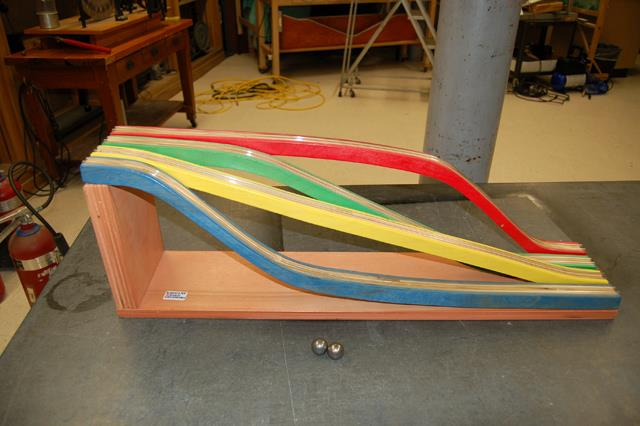
\includegraphics[scale=0.5]{FourFrictionless.png}
\end{center}
\end{textblock*}
\newpage
\begin{TeacherMargin}
\begin{center}
	\large
	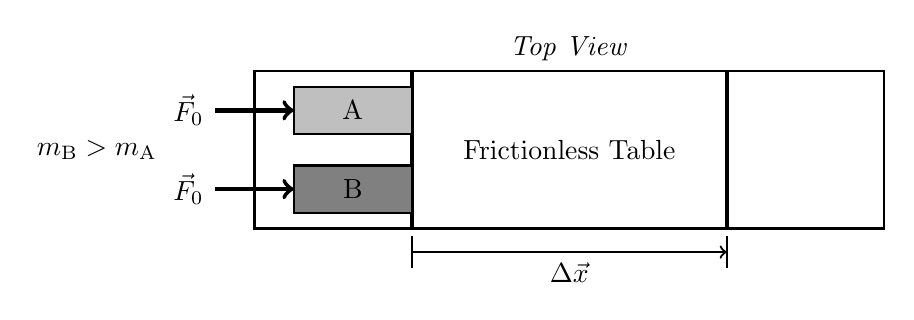
\begin{tikzpicture}
		\draw[thick] (0,-1) rectangle (8,1);
		\draw[ultra thick] (2,1) -- (2,-1);
		\node[anchor=south] at (4,1) {\textit{Top View}};
		\node at (4,0) {Frictionless Table};
		\draw[thick] (2,-1.1) -- (2,-1.5);
		\draw[ultra thick] (6,1) -- (6,-1);
		\draw[thick] (6,-1.1) -- (6,-1.5);
		\draw[thick,->] (2,-1.3) -- (4,-1.3) node[anchor=north] {$\Delta\vec{x}$} -- (6,-1.3);
		\draw[thick,color=black,fill=lightgray] (0.5,0.2) rectangle (2,0.8);
		\node at (1.25,0.5) {A};
		\draw[ultra thick,->] (-0.5,0.5) node[anchor=east] {$\vec{F}_{0}$} -- (0.5,0.5);
		\draw[thick,color=black,fill=gray] (0.5,-0.2) rectangle (2,-0.8);
		\node at (1.25,-0.5) {B};
		\draw[ultra thick,->] (-0.5,-0.5) node[anchor=east] {$\vec{F}_{0}$} -- (0.5,-0.5);
		\node at (-2,0) {$m_{\text{B}}>m_{\text{A}}$};
	\end{tikzpicture}
\end{center}
\textbf{Three Students} \\
A brief recap of what the students said is given in black, and the colored text discusses their logic.
\begin{enumerate}[(1)]
	\item Same force, $m_{\text{B}}>m_{\text{A}}$, therefore $m_{\text{A}}$ goes faster than $m_{\text{B}}$. \\
	{\color{blue}True by application of Newton's second law.} \\
	$\vec{p}=m\vec{v}$ {\color{blue} True (definition of momentum).}
	\item Speed compensates for mass, so $p_{\text{A},f} = p_{\text{B},f}$. \\
	{\color{violet}False. $m_{\text{A}}$ goes faster, so B will take longer to travel between the two marks. Symbolically, this can be written as $\Delta t_{\text{A}} < \Delta t_{\text{B}}$. $\vec{J} = \int_{t_{i}}^{t_{f}}\vec{F}^{net}dt$, so for the same force over these two different times, $J_{\text{A}} < J_{\text{B}}$, and since $p_{i}=0$ for both, this means $p_{\text{A},f} < p_{\text{B},f}$.}
	\item $K$ is proportional to $m$ and to $v^{2}$, so a bigger speed will have more effect than a smaller mass, thus $K_{\text{A}}>K_{\text{B}}$. \\
	{\color{violet} False. $W = \int_{\vec{r}_{i}}^{\vec{r}_{f}}\vec{F}\cdot d\vec{r}$ means $W_{\text{A}} = W_{\text{B}}$, as the blocks have the same force and displacement. The work-energy theorem then tells us that $K_{\text{A}}=K_{\text{B}}$.} \\
	{\color{violet}Also, note that $K=\frac{1}{2}mv^{2}=\frac{p^{2}}{2m}$, so if $K_{\text{A}} = K_{\text{B}}$, then}
	\begin{align*}
		\color{violet}
		\frac{p_{\text{A}}^{2}}{2m_{\text{A}}} = \frac{p_{\text{B}}^{2}}{2m_{\text{B}}},
	\end{align*}
	{\color{violet}which can be rearranged to get}
	\begin{align*}
		\color{violet}
		\frac{m_{\text{A}}}{m_{\text{B}}} = \frac{p_{\text{A}}^{2}}{p_{\text{B}}^{2}}.
	\end{align*}
	{\color{violet}Since $\frac{m_{\text{A}}}{m_{\text{B}}} < 1$, this tells us that $p_{\text{A}}<p_{\text{B}}$, giving extra confirmation that (2) is wrong.}
\end{enumerate}
\end{TeacherMargin}
\begin{PresentSpace}
\vspace{-10pt}
\section*{S8-4: Carts on a Track}
\vspace{-10pt}
\begin{itemize}
	\large
	\item Two carts, A and B, are initially at rest on a level, frictionless table. A constant force of magnitude $F_{0}$ is exerted on each cart as it travels between two marks. Cart B has a greater masss than cart A.
	\begin{center}
		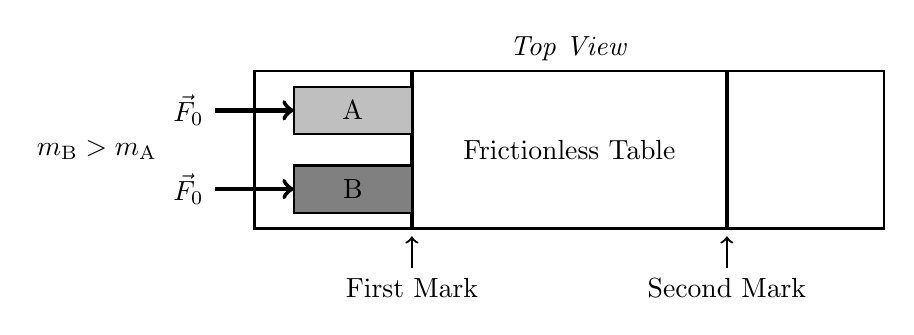
\begin{tikzpicture}
			\draw[thick] (0,-1) rectangle (8,1);
			\draw[ultra thick] (2,1) -- (2,-1);
			\node[anchor=south] at (4,1) {\textit{Top View}};
			\node at (4,0) {Frictionless Table};
			\draw[thick,<-] (2,-1.1) -- (2,-1.5) node[anchor=north] {First Mark};
			\draw[ultra thick] (6,1) -- (6,-1);
			\draw[thick,<-] (6,-1.1) -- (6,-1.5) node[anchor=north] {Second Mark};
			\draw[thick,color=black,fill=lightgray] (0.5,0.2) rectangle (2,0.8);
			\node at (1.25,0.5) {A};
			\draw[ultra thick,->] (-0.5,0.5) node[anchor=east] {$\vec{F}_{0}$} -- (0.5,0.5);
			\draw[thick,color=black,fill=gray] (0.5,-0.2) rectangle (2,-0.8);
			\node at (1.25,-0.5) {B};
			\draw[ultra thick,->] (-0.5,-0.5) node[anchor=east] {$\vec{F}_{0}$} -- (0.5,-0.5);
			\node at (-2,0) {$m_{\text{B}}>m_{\text{A}}$};
		\end{tikzpicture}
	\end{center}
	\item Three students discuss the final momentum and kinetic energy of each cart.
	\begin{enumerate}[(1)]
		\item \textit{``Since the same force is exerted on both carts, the cart with the smaller mass will move quickly, while the cart with the larger mass will move slowly. The momentum of each cart is equal to its mass times its velocity.''}
		\item \textit{``This must mean that the speed compensates for the mass and the two carts have equal final momenta.''}
		\item \textit{``I was thinking about the kinetic energies. Since the velocity is squared to get the kinetic energy, but mass isn't, the cart with the bigger speed must have more kinetic energy.''}
	\end{enumerate}
	\item Do you agree or disagree with the statements made by each student?
	\item Which cart takes longer to travel between the two marks? Explain your reasoning.
	\item Determine if the magnitude of the final momentum of cart A is \textit{greater than}, \textit{less than}, or \textit{equal to} that of cart B.
	\item Determine if the final kinetic energy of cart A is \textit{greater than}, \textit{less than}, or \textit{equal to} that of cart B.
	\item Reflect on your initial thoughts about the three students above.
\end{itemize}
\begin{center}
	\large
	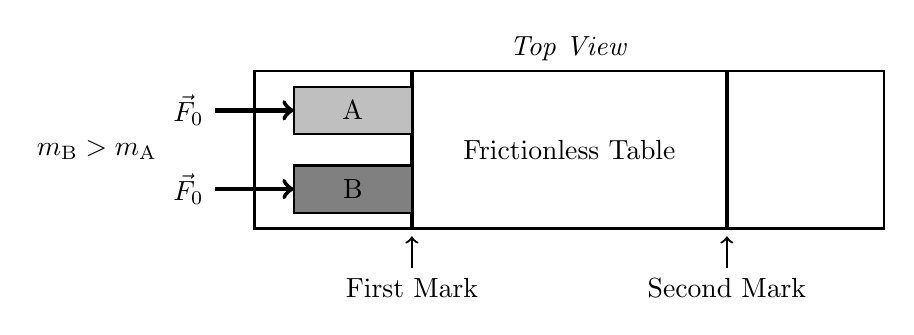
\begin{tikzpicture}
		\draw[thick] (0,-1) rectangle (8,1);
		\draw[ultra thick] (2,1) -- (2,-1);
		\node[anchor=south] at (4,1) {\textit{Top View}};
		\node at (4,0) {Frictionless Table};
		\draw[thick,<-] (2,-1.1) -- (2,-1.5) node[anchor=north] {First Mark};
		\draw[ultra thick] (6,1) -- (6,-1);
		\draw[thick,<-] (6,-1.1) -- (6,-1.5) node[anchor=north] {Second Mark};
		\draw[thick,color=black,fill=lightgray] (0.5,0.2) rectangle (2,0.8);
		\node at (1.25,0.5) {A};
		\draw[ultra thick,->] (-0.5,0.5) node[anchor=east] {$\vec{F}_{0}$} -- (0.5,0.5);
		\draw[thick,color=black,fill=gray] (0.5,-0.2) rectangle (2,-0.8);
		\node at (1.25,-0.5) {B};
		\draw[ultra thick,->] (-0.5,-0.5) node[anchor=east] {$\vec{F}_{0}$} -- (0.5,-0.5);
		\node at (-2,0) {$m_{\text{B}}>m_{\text{A}}$};
	\end{tikzpicture}
\end{center}
\end{PresentSpace}
\newpage
\begin{TeacherMargin}

\end{TeacherMargin}
\begin{PresentSpace}
\section*{Main Ideas}
\begin{itemize}
	\item The work-energy and impulse-momentum theorems can be used to solve a broad array of problems.
\end{itemize}
\end{PresentSpace}
\end{document}